%%%%%%%%%%%%%%%%%%%%%%%%%%%%%%%%%%%%%%%%%%%%%%%%%%%%%%%%%%%%
%%%%%%%%%%%%%%%%%%%%%%% preamble %%%%%%%%%%%%%%%%%%%%%%%%%%%
%%%%%%%%%%%%%%%%%%%%%%%%%%%%%%%%%%%%%%%%%%%%%%%%%%%%%%%%%%%%

\documentclass[compress,red,12pt]{beamer}
\mode<presentation>
%
% Beamer default paper size is 128mm by 96mm
%

\usetheme{Frankfurt}
% other themes: AnnArbor, Antibes, Bergen, Berkeley, Berlin,
%               Boadilla, boxes, CambridgeUS, Copenhagen,
%               Darmstadt, default, Dresden, Frankfurt, Goettingen,
%               Hannover, Ilmenau, JuanLesPins, Luebeck, Madrid, Maloe,
%               Marburg, Montpellier, PaloAlto, Pittsburg, Rochester,
%               Singapore, Szeged, classic

\usecolortheme{seahorse}
% color themes: albatross, beaver, beetle, crane, default, dolphin, dov,
%               fly, lily, orchid, rose, seagull, seahorse, sidebartab,
%               structure, whale, wolverine

\usefonttheme{structurebold}
% font themes: default, professionalfonts, serif, structurebold,
%               structureitalicserif, structuresmallcapsserif

%
% uncomment to go automatically to full screen
%
%\hypersetup{pdfpagemode=FullScreen}

% define your own colors:
\definecolor{Red}{rgb}{1,0,0}
\definecolor{Blue}{rgb}{0,0,1}
\definecolor{Green}{rgb}{0,1,0}
\definecolor{magenta}{rgb}{1,0,.6}
\definecolor{lightblue}{rgb}{0,.5,1}
\definecolor{lightpurple}{rgb}{.6,.4,1}
\definecolor{gold}{rgb}{.6,.5,0}
\definecolor{orange}{rgb}{1,0.4,0}
\definecolor{hotpink}{rgb}{1,0,0.5}
\definecolor{newcolor2}{rgb}{.5,.3,.5}
\definecolor{newcolor}{rgb}{0,.3,1}
\definecolor{newcolor3}{rgb}{1,0,.35}
\definecolor{darkgreen1}{rgb}{0, .35, 0}
\definecolor{darkgreen}{rgb}{0, .6, 0}
\definecolor{darkred}{rgb}{.75,0,0}

\xdefinecolor{olive}{cmyk}{0.64,0,0.95,0.4}
\xdefinecolor{purpleish}{cmyk}{0.75,0.75,0,0}

% can also choose different themes for the "inside" and "outside"

% \usepackage{beamerinnertheme_______}
% inner themes include circles, default, inmargin, rectangles, rounded
\useinnertheme{circles}

% \usepackage{beamerouterthemesmoothbars}
% outer themes include default, infolines, miniframes, shadow, sidebar,
%               smoothbars, smoothtree, split, tree
\useoutertheme{miniframes}

% to have the same footer on all slides
%\setbeamertemplate{footline}[text line]{STUFF HERE!}
%\setbeamertemplate{footline}[text line]{} % makes the footer EMPTY
%\setbeamertemplate{footline}{\scriptsize{\vspace*{0.4cm}\hspace*{0.3cm}\insertframenumber}} 

%
% Automatic Outline
%
\AtBeginSection[section]
{
  \begin{frame}
    \frametitle{Outline}
    \tableofcontents[sectionstyle=show/shaded,subsectionstyle=show/show/hide]
  \end{frame}
}

%
% For speed up of compilation
%
\includeonlyframes{current}


%
% include packages
%
\usepackage[latin1]{inputenc}
\usepackage[small]{caption}
\captionsetup{labelformat=empty, labelsep=none}
\usepackage{graphicx}
\graphicspath{{./images/}}
\usepackage{bm}
\usepackage{fancybox}
\usepackage{multimedia}
\usepackage{amsmath}
\usepackage{amssymb}
\usepackage{tikz}
\usetikzlibrary{arrows,shapes}
\tikzstyle{every picture}+=[remember picture]
\tikzstyle{na} = [baseline=-.5ex]
\usepackage{cancel}

%%%%%%%%%%%%%%%%%%%%%%%%%%%%%%%%%%%%%%%%%%%%%%%%%%%%%%%%%%%%
%%%%%%%%%%%%%%%%%% Custom Commands I Use  %%%%%%%%%%%%%%%%%%
%%%%%%%%%%%%%%%%%%%%%%%%%%%%%%%%%%%%%%%%%%%%%%%%%%%%%%%%%%%%

\newcommand{\OpSphere}{\bm{\mathcal{S}}}
\newcommand{\OpRot}{\bm{\mathcal{R}}}
\newcommand{\OpDistance}{\bm{\mathcal{D}}}
\newcommand{\OpCumsum}{\bm{\mathcal{C}}}
\newcommand{\OpInt}{\bm{\mathcal{I}}}
\newcommand{\OpCamera}{\bm{\mathcal{P}}}
\newcommand{\OpDiag}[1]{\mathrm{diag}\left\{#1\right\}}
\newcommand{\Grad}[1]{\bm{\triangledown_{#1}}}
\newcommand{\argmin}{\operatornamewithlimits{argmin}}
\newcommand{\curly}[1]{\left\{#1\right\}}
\newcommand{\roundy}[1]{\left(#1\right)}
\newcommand{\recty}[1]{\left[#1\right]}
\newcommand{\PartDeriv}[2]{\frac{\partial{#1}}{\partial{#2}}}
\newcommand{\vect}[1]{\bm{#1}}
\newcommand{\mat}[1]{\bm{#1}}
\newcommand{\transpose}[1]{{#1}^\intercal}
\newcommand{\derivsym}[1]{\,d{#1}}

%%%%%%%%%%%%%%%%%%%%%%%%%%%%%%%%%%%%%%%%%%%%%%%%%%%%%%%%%%%%
%%%%%%%%%%%%%%%%%% title page information %%%%%%%%%%%%%%%%%%
%%%%%%%%%%%%%%%%%%%%%%%%%%%%%%%%%%%%%%%%%%%%%%%%%%%%%%%%%%%%

\title[3D Aerosol Recovery]{
  Lightfield Analysis and Recovery of the Atmosphere
}

\author[Amit Aides]{
  Student: Amit Aides \\
  Supervisor: Prof. Yoav Y. Schechner
}

\date{12 September 2013}

%%%%%%%%%%%%%%%%%%%%%%%%%%%%%%%%%%%%%%%%%%%%%%%%%%%%%%%%%%%%
%%%%%%%%%%%%%%%%%%%%%%% begin %%%%%%%%%%%%%%%%%%%%%%%%%%%%%%
%%%%%%%%%%%%%%%%%%%%%%%%%%%%%%%%%%%%%%%%%%%%%%%%%%%%%%%%%%%%

\begin{document}

\begin{frame}
  \titlepage
\end{frame}

%%%%%%%%%%%%%%%%%%%%%%%%%%%%%%%%%%%%%%%%%%%%%%%%%%%%%%%%%%%%
%%%%%%%%%%%%%%%%%%%%%%%%%%%%%%%%%%%%%%%%%%%%%%%%%%%%%%%%%%%%

\section{Introduction}

%%%%%%%%%%%%%%%%%%%%%%%%%%%%%%%%%%%%%%%%%%%%%%%%%%%%%%%

\subsection{Motivation}

\begin{frame}{Motivation}
  \setbeamercovered{transparent}
  \begin{itemize}
  \item<1-> Fine solid particles or liquid droplets suspended in the
    atmosphere
  \item<2-> Affects the health of Earth's inhabitants
  \item<3-> Affects Earth's climate
  \end{itemize}
  \begin{overlayarea}{\textwidth}{6cm}
    \begin{center}
      \includegraphics<1>[width=\columnwidth]{images/aerosol_micrographs.jpg}
      \includegraphics<2>[height=4cm]{images/shenzen_haze.jpg}
      \includegraphics<3>[height=4cm]{images/radiation_budget.jpg}
    \end{center}    
  \end{overlayarea}
  \begin{flushright}
    \only<1-2> {\tiny images taken from
      http://earthobservatory.nasa.gov/Features/Aerosols/}
    \only<3> {\tiny image taken from
      http://calipsooutreach.hamptonu.edu/index.html}
  \end{flushright}
\end{frame}

\begin{frame}{Aerosols Distribution is 3D}
  \begin{itemize}
    \item Eyjafjallaj\"{o}kull Eruption in 2010
  \end{itemize}
  \begin{center}
    \includegraphics<1>[height=6cm]{images/1024px-Eyjafjallajokull_volcano_plume.jpg}
  \end{center}
  \begin{flushright}
    \only<1> {\tiny image taken from http://www.wikipedia.com/}
  \end{flushright}
\end{frame}

\begin{frame}{Aerosols Distribution is 3D}
  \begin{center}
    \includegraphics<1>[height=7cm]{images/Volcanic_Lavender.jpg}
    \includegraphics<2>[height=7cm]{images/volcano-airport.jpg}
  \end{center}
  \begin{flushright}
    \only<1> {\tiny image taken from http://www.wikipedia.com/}
    \only<2> {\tiny image taken from
http://www.metrolic.com/eyjafjallajokull-is-dormant...for-the-moment-2042/}
  \end{flushright}
\end{frame}

%%%%%%%%%%%%%%%%%%%%%%%%%%%%%%%%%%%%%%%%%%%%%%%%%%%%%%%

\subsection{Aerosols Recovery Methods}

\begin{frame}{Existing Methods}
  \begin{itemize}
  \item<1> MISR - Multi-angle Imaging SpectroRadiometer
  \end{itemize}
  \begin{center}
    \includegraphics<1>[width=\columnwidth]{images/misr.pdf}
  \end{center}
  \begin{flushright}
    \only<1> {\tiny images taken from http://www-misr.jpl.nasa.gov/}
  \end{flushright}
\end{frame}

\begin{frame}{Common Atmospheric Models}
  \begin{itemize}
  \item<1> 1D or 2D models
  \end{itemize}
  \begin{center}
    \includegraphics<1>[height=6cm]{images/atmosphere_layer.jpg}
  \end{center}
  \begin{flushright}
    \only<1> {\tiny image taken from the Stratospheric Ozone Electronic Textbook}
  \end{flushright}
\end{frame}

\begin{frame}{Existing Methods}
  \begin{itemize}
  \item<1> LIDAR - Light Detection And Ranging
  \end{itemize}
  \begin{center}
    \includegraphics<1>[width=\columnwidth]{images/lidar.pdf}
  \end{center}
  \begin{flushright}
    \only<1> {\tiny images taken from
      http://jp.hamamatsu.com/en/rd/technology/energy/lidar.html}
  \end{flushright}
\end{frame}

%%%%%%%%%%%%%%%%%%%%%%%%%%%%%%%%%%%%%%%%%%%%%%%%%%%%%%%

\subsection{Suggested Method}

\begin{frame}{Multi-angle Tomographic Reconstruction}
  \setbeamercovered{transparent}
  \begin{itemize}
  \item <2-> Multi-angle imaging from the ground
  \end{itemize}
  \begin{center}
    \only<1>
    {\includegraphics[height=5cm]{images/camera_network-0.png}}
    \only<2>
    {\includegraphics[height=5cm]{images/camera_network-1.png}}
  \end{center}
\end{frame}

%%%%%%%%%%%%%%%%%%%%%%%%%%%%%%%%%%%%%%%%%%%%%%%%%%%%%%%

\subsection{Related Work}

\begin{frame}{$SO_2$}
  
\end{frame}

\begin{frame}{Optical Tomography}
  
\end{frame}


%%%%%%%%%%%%%%%%%%%%%%%%%%%%%%%%%%%%%%%%%%%%%%%%%%%%%%%%%%%%
%%%%%%%%%%%%%%%%%%%%%%%%%%%%%%%%%%%%%%%%%%%%%%%%%%%%%%%%%%%%

\section{Theory}

%%%%%%%%%%%%%%%%%%%%%%%%%%%%%%%%%%%%%%%%%%%%%%%%%%%%%%%

\subsection{Radiative Transfer}

\begin{frame}{Optical Depth}
  \setbeamercovered{transparent}
  \begin{overlayarea}{\textwidth}{3cm}
    \begin{itemize}
    \item <1-> Light is attenuated according to the {\em Beer-Lambert}
      law
    \item <2> Optical depth is a measure of transparency
    \end{itemize}
  \end{overlayarea}
  \begin{overlayarea}{\textwidth}{3cm}
    \begin{center}
      \only<1> {
        \includegraphics<1>[width=0.5\columnwidth]{images/beer_lambert.pdf}
      }
      \only<2> {
        \begin{align*}
          \tau = \sigma \int_{0}^x N(\tilde{x})\derivsym{\tilde{x}}
        \end{align*}
      }
    \end{center}
  \end{overlayarea}
\end{frame}

\begin{frame}{Scattering}
  \begin{itemize}
  \item Rayleigh - particles smaller then wavelength
  \item Mie - particles bigger then wavelength
  \end{itemize}
  \begin{center}
    \shadowbox{\includegraphics[height=4cm]{images/Mie_Rayleigh.jpg}}
  \end{center}
\end{frame}

\begin{frame}{Boltzman Equation}
  
\end{frame}

%%%%%%%%%%%%%%%%%%%%%%%%%%%%%%%%%%%%%%%%%%%%%%%%%%%%%%%

\subsection{Approximated Solutions}

\begin{frame}{Single Scattering}
  
\end{frame}

%%%%%%%%%%%%%%%%%%%%%%%%%%%%%%%%%%%%%%%%%%%%%%%%%%%%%%%

\subsection{Inverse Problem}

\begin{frame}{Numerical}
  
\end{frame}

%%%%%%%%%%%%%%%%%%%%%%%%%%%%%%%%%%%%%%%%%%%%%%%%%%%%%%%%%%%%
%%%%%%%%%%%%%%%%%%%%%%%%%%%%%%%%%%%%%%%%%%%%%%%%%%%%%%%%%%%%

\section{Current PhD Research: Ongoing}

%%%%%%%%%%%%%%%%%%%%%%%%%%%%%%%%%%%%%%%%%%%%%%%%%%%%%%%

\subsection{Image formation using the single-scattering model}

\begin{frame}{Model}
  \begin{columns}[c]
    \column{0.5\columnwidth}
    \setbeamercovered{transparent}
    \begin{itemize}
    \item <1-2> Atmosphere volume
    \item <1-2> Voxel - Volume Element
    \item <3-4> Light is attenuated due to scattering and absorption
    \item <3-5> Light scatters only once between source and viewer
    \item <6> Simple forward model
    \item <6> No Multi-Scattering
    \end{itemize}
    \column{0.5\columnwidth}
    \begin{overlayarea}{\columnwidth}{8cm}
      \only<1> {\centerline{\includegraphics[width=\columnwidth]
          {images/atmo_settings3D1.pdf}}}
      \only<2> {\centerline{\includegraphics[width=\columnwidth]
          {images/atmo_settings3D2.pdf}}}
      \only<3> {\centerline{\includegraphics[width=\columnwidth]
          {images/atmo_settings3D3.pdf}}}
      \only<4> {\centerline{\includegraphics[width=\columnwidth]
          {images/atmo_settings3D4.pdf}}}
      \only<5> {\centerline{\includegraphics[width=\columnwidth]
          {images/atmo_settings3D5.pdf}}}
      \only<6> {\centerline{\includegraphics[width=\columnwidth]
          {images/atmo_settings3D6.pdf}}}
    \end{overlayarea}
\end{columns}
\end{frame}

\begin{frame}{Image Formation Model}
  \begin{columns}[c]

    \column{0.7\textwidth}

    \begin{itemize}
    \item <3-> Attenuation \tikz[na] \node[coordinate] (s2) {};
    \item <4-> Scattering \tikz[na] \node[coordinate] (s3) {};
    \end{itemize}

    % \small
    \footnotesize
    \begin{align*}
      \mathrm{I} &= \\
      & \tikz[baseline]{
        \node[fill=blue!20,anchor=base,rounded corners=2pt]
        (d1) {$\mathrm{L}^{\rm TOA}$}; } \,
      \tikz[baseline]{ \node[fill=red!20,anchor=base,rounded corners=2pt]
        (d4) {$\OpCamera$}; }
      \curly{\roundy{
          \tikz[baseline]{ \node[fill=green!20,anchor=base,rounded corners=2pt]
            (d3) {$\vect{\alpha}^{\rm aerosol} + \vect{\alpha}^{\rm air}$}; } }  \odot 
        \tikz[baseline]{ \node[fill=yellow!20,anchor=base,rounded corners=2pt]
          (d2) {$\exp^{-(\vect{\tau}^{\rm aerosol} + \vect{\tau}^{\rm air})}$}; } }
    \end{align*}
    \normalsize

    \begin{itemize}
    \item <2-> Sun \tikz[na] \node[coordinate] (s1) {}; luminance 
    \item <5-> Camera projection \tikz[na] \node[coordinate] (s4) {};
    \end{itemize}

    \begin{tikzpicture}[overlay]                  \pause
      \path[->] (s1) edge [bend right] (d1);     \pause
      \path[->] (s2) edge [bend left] (d2);    \pause
      \path[->] (s3) edge [bend left] (d3); \pause
      \path[->] (s4) edge [bend right] (d4); \pause
    \end{tikzpicture}

    \column{0.3\textwidth}

    \begin{overprint}
      \only<1-2> {\centerline{\includegraphics[width=\columnwidth]
          {images/atmo_settings3D2.pdf}}}
      \only<3> {\centerline{\includegraphics[width=\columnwidth]
          {images/atmo_settings3D3.pdf}}}
      \only<4-> {\centerline{\includegraphics[width=\columnwidth]
          {images/atmo_settings3D5.pdf}}}
    \end{overprint}

  \end{columns}
\end{frame}

\begin{frame}{Synthesized Examples}
  \begin{columns}[C]
    \begin{column}{.7\textwidth}
      \begin{overlayarea}{\columnwidth}{8cm}
        \only<1>
        {\centerline{\includegraphics[height=7cm]{images/single_img1.pdf}}}
        \only<2>
        {\centerline{\includegraphics[height=7cm]{images/single_img2.pdf}}}
        \only<3>
        {\centerline{\includegraphics[height=7cm]{images/single_img3.pdf}}}
        \only<4>
        {\centerline{\includegraphics[height=7cm]{images/single_img4.pdf}}}
        \only<5>
        {\centerline{\includegraphics[height=7cm]{images/single_img5.pdf}}}
        \only<6>
        {\centerline{\includegraphics[height=7cm]{images/single_img6.pdf}}}
        \only<7>
        {\centerline{\includegraphics[height=7cm]{images/single_img7.pdf}}}
        \only<8>
        {\centerline{\includegraphics[height=7cm]{images/single_img8.pdf}}}
        \only<9>
        {\centerline{\includegraphics[height=7cm]{images/single_img9.pdf}}}
      \end{overlayarea}
    \end{column}
    \begin{column}{.3\textwidth}
      \begin{figure}
        \centering
        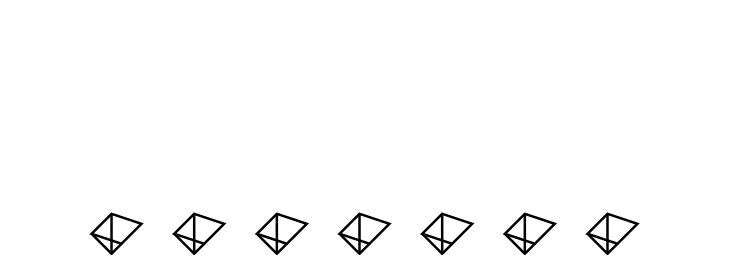
\includegraphics[width=\columnwidth]{images/atmo3d.pdf}
      \end{figure}
    \end{column}
  \end{columns}
\end{frame}

%%%%%%%%%%%%%%%%%%%%%%%%%%%%%%%%%%%%%%%%%%%%%%%%%%%%%%%

\subsection{Monte Carlo}

\begin{frame}{Monte Carlo}
  \begin{figure}
    \centering
    \begin{overprint}
      \only<1>
      {\centerline{\def\svgwidth{0.5\linewidth}\small{\input{images/mc_method.pdf_tex}}}}
      \only<2>
      {\centerline{\includegraphics[height=7cm]{images/mc_result.pdf}}}
      \only<3>
      {\centerline{\def\svgwidth{0.5\linewidth}\small{\input{images/cross_section.pdf_tex}}}}
    \end{overprint}
  \end{figure}
\end{frame}

%%%%%%%%%%%%%%%%%%%%%%%%%%%%%%%%%%%%%%%%%%%%%%%%%%%%%%%

\subsection{Inverse Problem}

\begin{frame}{Inverse Problem}
  \begin{block}{Problem}
    Given a set of captured images, calculate the underlying aerosol
    distribution
  \end{block}
\end{frame}

\begin{frame}{Formulation}
  \setbeamercovered{transparent}
  \begin{block}{Objective Function}
    \begin{align*}
      {\rm minimize} \, f =  \sum_{\mbox{all images}} \left| \left( \begin{array}{c}\mbox{measured} \\ \mbox{image} \end{array} \right) - \left( \begin{array}{c}\mbox{modeled} \\ \mbox{image} \end{array} \right) \right|
    \end{align*}

    \onslide<2->{
      \begin{itemize}
      \item Formally
      \begin{align*}
        f &= \sum_{c=1}^{N_{\rm cams}} ||\mathrm{I}_c-\hat{\mathrm{I}}_c(\mat{A})||_2^2 \\
        &\hat{\mat{A}}^{\rm aerosol} = \argmin_{\mat{A}} f
      \end{align*}

      \end{itemize}
    }
  \end{block}

\end{frame}

\begin{frame}{Challenge}
  \begin{figure}
    \centering
    \centerline{\includegraphics[height=7cm]{images/voxels3.pdf}}
  \end{figure}
\end{frame}

\begin{frame}{Jacobian (Differentiation)}
  \setbeamercovered{transparent}
  \begin{block}{Gradient}
    \begin{align*}
      \Grad{\mat{A}} f = -2\sum_{c=1}^{N_{\rm cams}}
      \transpose{\left[\mat{J}_{\hat{\vect{i}}_c}(\mat{A})\right]}(\mathrm{I}_c-\hat{\mathrm{I}}_c)
    \end{align*}
  \end{block}
  \pause
  \begin{block}{Jacobian Equation}
    \begin{align*}
      \mat{J}_{\hat{\vect{i}}_c}(\mat{A}) &= \mathrm{L}^{\rm TOA}\,
      \Big( \sigma^{\rm aerosol} \, \varpi \, \OpDiag{P^{\rm
          aerosol}(\vect{\mu}_c)} - \nonumber \\
      &\quad \transpose{\OpDistance} \OpDiag{ (\vect{\alpha}^{\rm
          aerosol}_c + \vect{\alpha}^{\rm air}_c )} \Big)
      \OpDiag{\exp^{-(\vect{\tau}^{\rm aerosol}_c + \vect{\tau}^{\rm
            air}_c)}}\transpose{\OpCamera}
    \end{align*}
  \end{block}
\end{frame}

\begin{frame}{Parallelization}
  \begin{itemize}
  \item Processed using a computer cluster
  \item Each synthetic camera processed on a separate core
  \item Total 95 synthetic cameras
  \item A couple of hours to reconstruct 250K voxels
  \end{itemize}
\end{frame}

\subsection{Results}

\begin{frame}{Reconstruction Results}
  \begin{overlayarea}{\textwidth}{5cm}
    \only<1>
    {
      \centerline{Original Atmospheres}
      \centerline{\def\svgwidth{1.15\linewidth}\footnotesize{\input{images/atmo3d_original.pdf_tex}}}
    }
    \only<2>
    {
      \centerline{Reconstruction from Single-scattering Simulations}
      \centerline{\def\svgwidth{1.15\linewidth}\footnotesize{\input{images/atmo3d_single.pdf_tex}}}
    }
    \only<3>
    {
      \centerline{Reconstruction from Multi-scattering Simulations}
      \centerline{\def\svgwidth{1.15\linewidth}\footnotesize{\input{images/atmo3d_mc.pdf_tex}}}
    }
  \end{overlayarea}
  \centerline{\footnotesize Color represents aerosol density. The
    density units are $10^{6}~{\rm particles}/{\rm m}^3.$}
\end{frame}


%%%%%%%%%%%%%%%%%%%%%%%%%%%%%%%%%%%%%%%%%%%%%%%%%%%%%%%%%%%%
%%%%%%%%%%%%%%%%%%%%%%%%%%%%%%%%%%%%%%%%%%%%%%%%%%%%%%%%%%%%

\section{Further Research Directions}

%%%%%%%%%%%%%%%%%%%%%%%%%%%%%%%%%%%%%%%%%%%%%%%%%%%%%%%%%%%%
%%%%%%%%%%%%%%%%%%%%%%%% end %%%%%%%%%%%%%%%%%%%%%%%%%%%%%%%
%%%%%%%%%%%%%%%%%%%%%%%%%%%%%%%%%%%%%%%%%%%%%%%%%%%%%%%%%%%%

\end{document}

